\documentclass[11pt]{article}
\usepackage[a4paper,margin=0.85in]{geometry}
\usepackage[T1]{fontenc}
\usepackage{lmodern}
\usepackage{microtype}
\usepackage{graphicx}
\usepackage{booktabs}
\usepackage{amsmath}
\usepackage{amssymb}
\usepackage{hyperref}
\usepackage{xcolor}
\usepackage{float}
\usepackage{array}
\usepackage{adjustbox}

\hypersetup{
    colorlinks=true,
    linkcolor=black,
    citecolor=black,
    urlcolor=blue
}

\title{SAiDL Summer Assignment 2026\\Reinforcement Learning Report}
\author{Krish Sachdev}
\date{7 June 2026}

\begin{document}
\maketitle

\begin{abstract}
This report studies whether a causal Transformer policy can use short-term temporal memory better than a memoryless MLP policy in online reinforcement learning. I implemented TD3 on Hopper-v5, replaced the actor with a causal Transformer over the last $L$ observation-action pairs, swept $L \in \{4,8,16,32\}$, and then tested both policy classes under hidden velocities, observation noise, delayed rewards, and a learned preference reward model. The final required comparison uses 20 successful W\&B runs created between 2026-05-22T17:30:00+00:00 and 2026-05-29T17:30:00+00:00. The strongest final "required" run was \texttt{rl\_p1\_mlp\_seed44} with return 3540.2; the strongest "required" checkpoint was \texttt{rl\_p1\_tr\_L4\_seed42} with return 3596.1 at step 680000. I also report the finished bonus runs available in the current W\&B export: hidden-velocity positional ablations with a history-conditioned critic and a combined hidden-velocity/noise/delayed-reward POMDP. The best bonus final return is RoPE with the history-conditioned critic (1109.3), while sinusoidal encoding has the highest bonus peak (1567.0) but a larger best-final gap. Empirically, Transformer memory can help in delayed-reward and full-observation settings, and the bonus runs show that critic conditioning matters substantially under hidden velocity, but several curves still show late deterioration after an earlier good policy.
\end{abstract}

\section{Task Requirements and Scope}

The assignment asks for TD3 on Hopper-v5 over three MLP seeds, a Transformer actor that attends over a sliding window of the last $L$ observation-action pairs, a context-length sweep over $L \in \{4,8,16,32\}$, independent partial-observability modifications, an RLHF-style learned reward model, and attention analysis for trained Transformer agents~\cite{saidl2026}. All required non-bonus runs in the runner were completed successfully in the final W\&B window, and the later attention-analysis runner completed the entropy-history and five-episode rollout analysis for both the fully observable and hidden-velocity Transformer policies. Bonus experiments are reported in a separate section so the required-suite conclusions remain tied to the original required suite, while the newer bonus evidence can be compared on its own terms.

For reproducibility, I keep two views of the run history. Final metric comparisons use the latest finished run for each exact experiment when a completed run exists. The attempt-inclusive run export keeps every non-failed run from the final three-week W\&B window, including crashed runs, because many crashes were Kaggle session-limit interruptions that were later continued under the same experiment name. Runs whose W\&B state is exactly \texttt{failed} are excluded from these attempt-inclusive tables.

\begin{table}[!htbp]
\centering
\small
\caption{Requirement-level coverage against the RL section of the assignment PDF.}
\label{tab:assignment-checklist}
\resizebox{\textwidth}{!}{%
\begin{tabular}{lll}
\toprule
Assignment item & Status & Evidence used in this report \\
\midrule
TD3 MLP baseline, 3 seeds & Complete & rl\_p1\_mlp\_seed42/43/44, 1M steps \\
Transformer TD3, L sweep & Complete & L=4,8,16,32 final runs \\
Hidden velocities & Complete & MLP and Transformer runs \\
Observation noise & Complete & sigma=0.1 and sigma=0.3, both agents \\
Delayed rewards & Complete & K=10 and K=30, both agents \\
RLHF-style learned reward & Complete with caveat & rl\_p2\_rlhf\_tr\_seed42 plus reward-model loss; contamination caveat discussed below \\
Attention analysis & Complete & jx1lmi8i and lap7edb6 entropy histories plus 5-episode checkpoint rollouts \\
Bonus positional encoding ablation & Complete supplemental evidence & Latest finished learned/sinusoidal/RoPE hidden-velocity runs use the history-conditioned critic \\
Bonus combined POMDP & Complete supplemental evidence & \texttt{rl\_bonus\_combined\_L32\_stable\_seed42}, hidden velocity + noise 0.1 + delay K=10 \\
Bonus Algorithm Distillation & Not counted & No finished AD metric row in the current W\&B export \\
Bonus xLSTM policy & Not counted & No finished xLSTM metric row in the current W\&B export \\
\bottomrule
\end{tabular}
}
\end{table}

\subsection{Data Provenance}

The scalar results come from the W\&B project \href{https://wandb.ai/krishsachdev246-bits-pilani/saidl-rl}{saidl-rl}. The repository keeps the final report source, compiled PDF, and figures used for the analysis. Bonus evidence is exported separately under \path{rl/report/data/clean_rl_bonus_runs.csv} and \path{rl/report/tables}, including the exact-name latest-finished selection and the same-name instability comparison. The completed attention-analysis notebook artifacts are included under \path{rl/report/data} and \path{rl/report/figures}; these include W\&B entropy histories, checkpoint manifests, final lag weights, and five-episode rollout summaries.

\section{Method}

\subsection{TD3 Backbone}

The base learner is Twin Delayed Deep Deterministic Policy Gradient. The critic uses two Q-functions to reduce over-estimation bias, the target action is smoothed with clipped noise, and the actor is updated less frequently than the critic. The configuration followed the assignment's preferred regime: learning rate $3 \times 10^{-4}$, replay buffer size $10^6$, batch size 256, discount $\gamma=0.99$, soft target update rate $\tau=0.005$, policy delay 2, exploration noise 0.1, target noise 0.2, and random exploration for the first 25k steps.

\subsection{Policies}

The MLP baseline maps the current observation directly to a tanh-squashed action using two hidden layers. The Transformer actor instead receives a causal sequence of recent observation-action pairs. For the current timestep, the last action slot is zero-filled, causal self-attention prevents future leakage, and the final token representation is projected to the action. The Transformer uses two layers, four heads, embedding dimension 128, pre-layer normalisation, and a default context length $L=8$ unless overridden in the context sweep.

\subsection{Environment Modifications}

The full-observation baseline uses Hopper-v5. Hidden-velocity experiments remove velocity components from the observation vector, making the task partially observable. Noisy-observation experiments add Gaussian noise with $\sigma=0.1$ and $\sigma=0.3$. Delayed-reward experiments accumulate reward and expose it only every $K$ steps for $K=10$ and $K=30$. These modifications are applied independently, as requested, so each setting isolates one source of temporal uncertainty.

\subsection{Learned Reward Model}

For the RLHF-style run, trajectory segment pairs are sampled from replay. Labels are generated from ground-truth segment returns, and a Bradley-Terry objective trains a learned reward model. TD3 then stores learned reward predictions instead of environment rewards after the initial exploration phase. Ground-truth returns are used for preference labels and evaluation only.

\subsection{Evaluation Protocol}

Each run trains to 1,000,000 environment steps, evaluates every 10,000 steps, and averages each evaluation over 10 episodes. I report both final evaluation return and best checkpoint return. This distinction matters because off-policy actor-critic learning can reach a good policy before later critic drift, replay-distribution shift, or actor over-updating degrades performance.

\subsection{Bonus Stability Variant}

The later bonus reruns kept the Transformer actor but changed the critic-side information available during updates. Earlier positional-encoding bonus runs used a flat critic over the current transition, while the stabilized bonus runs logged \texttt{critic\_sequence\_context=1.0}, meaning the critic update used history-conditioned inputs aligned with the actor's temporal context. These runs also logged target-Q scale, target-Q clipping fraction, Q-gap diagnostics, and critic losses (the additions were made in an attempt to combat late-run instability). The report therefore compares the newest finished stabilized run for each exact experiment name against older finished attempts of the same name where such attempts exist.

\section{Execution Notes and Roadblocks}

The final execution was done on Kaggle with W\&B logging, with initial runs on a P100. Later GPU allocation constraints forced me to switch to running on 2xT4. This affects wall-clock runtime and throughput comparisons, but not the meaning of evaluation returns when code, seed, total steps, checkpoints, and configs are otherwise matched. Consequently, hardware labels are shown in the tables.

A separate resume issue appeared when a checkpoint saved from a T4 session was resumed on a P100 runtime. The failure was an \texttt{IndexError} inside \texttt{torch.cuda.set\_rng\_state\_all}, caused by restoring CUDA RNG states saved for a different GPU count/layout than the current runtime (because of the way I'd patched checkpoint saves). The fix I came up with during the run window was to continue the final suite on T4, matching the saved checkpoint environment. The final repository also guards CUDA RNG restoration by restoring only the first \texttt{torch.cuda.device\_count()} saved CUDA RNG states. This makes cross-layout continuation safer, although exact bitwise reproducibility is still not a meaningful promise after changing GPU layout.

Several intermediate runs crashed because of runtime limits or resume mismatches. Instead of discarding those partial runs, I keep a three-week attempt-inclusive export that includes both crashed and finished runs and excludes only W\&B state \texttt{failed}. Table~\ref{tab:attempt-inclusive} summarizes exact-name groups with more than one non-failed attempt; the full 51-row export is included as \path{rl/report/data/wandb_rl_runs_last3w_nonfailed.csv}.

\section{Debugging and Troubleshooting}

The main RL troubleshooting problem was keeping long Kaggle runs recoverable and making sure failed attempts did not contaminate the reported comparison. Table~\ref{tab:rl-debugging} records the major issues, their diagnoses, and the final handling used in the report and code.

\begin{table}[!htbp]
\centering
\small
\caption{RL debugging and troubleshooting log.}
\label{tab:rl-debugging}
\resizebox{\textwidth}{!}{%
\begin{tabular}{p{0.21\textwidth}p{0.35\textwidth}p{0.34\textwidth}}
\toprule
Issue & Diagnosis & Resolution and final status \\
\midrule
P100 queue and hardware switch & A runner notebook remained queued for roughly two hours on P100, while T4 allocation became available. This changed wall-clock runtime conditions but did not change the mathematical RL objective. & The final suite records hardware per run. Evaluation-return comparisons are kept separate from runtime-throughput comparisons, and T4/P100 runtime differences are treated as execution caveats rather than algorithmic evidence. \\
Cross-GPU checkpoint resume failure & T4 checkpoints could save CUDA RNG state for a different GPU layout than the later P100 runtime. Restoring all saved states produced an \texttt{IndexError}. & During execution, affected runs were resumed on matching T4 hardware. In the final code, CUDA RNG restoration is bounded by the current \texttt{torch.cuda.device\_count()}, so extra saved RNG states are ignored instead of crashing resume. \\
Attention runner config error & The attention rerun initially read \texttt{cfg.agent.context\_length}; the actual Transformer config stores this value under \texttt{cfg.agent.actor.context\_length}. Hydra struct mode therefore raised \texttt{ConfigAttributeError}. & The attention analysis path was revised to read the actor context length. The completed rerun produced entropy-vs-step histories, final lag weights, checkpoint manifests, and five-episode rollout summaries for full and hidden-velocity policies. \\
Interrupted duplicate runs & Several runs failed or crashed from runtime limits, resume mismatches, or notebook interruptions, but later runs with the same experiment name often continued or superseded them. Treating all interruptions as bad experiments would lose useful run-history evidence; treating them as independent finished experiments would double-count. & Runs with state \texttt{failed} are excluded. Crashed and finished runs from 2026-05-18 through 2026-06-07 are retained in the attempt-inclusive export. Main metric tables still use the latest finished run for an exact experiment name when a finished run exists. \\
Learned-reward ambiguity & The intended RLHF setup labels preference pairs using ground-truth segment returns. On code review, later replay entries can contain learned reward predictions, making later reward-model updates susceptible to self-reinforcing reward-model error. & The learned-reward result is reported as an implementation-level learned-reward baseline, not as a clean general claim about RLHF. The large gap versus ground-truth reward is interpreted with this caveat. \\
Best return much higher than final return & Many runs reached a strong policy before later deterioration. Reporting only final returns would hide learned capability; reporting only best returns would hide instability. & The report keeps both values. Final return is the strict end-of-run metric, best return measures peak learned performance, and the best-final gap is used as a stability diagnostic. \\
Bonus stability reruns & Early bonus positional runs stayed near 200--250 final return or peaked briefly and collapsed. The stability changes added target-Q diagnostics and, in the latest finished reruns, history-conditioned critic inputs. & The bonus section selects the newest finished run for each exact experiment name. Earlier same-name runs are retained as instability evidence instead of being mixed into the final metric table. \\
\bottomrule
\end{tabular}
}
\end{table}

\section{Run Coverage}

\begin{table}[!htbp]
\centering
\scriptsize
\caption{Selected successful required RL runs from the final W\&B window.}
\label{tab:selected-runs}
\resizebox{\textwidth}{!}{%
\begin{tabular}{lllllllllllll}
\toprule
Run & Part & Agent & Env & L & Final & Best & Best step & Gap & Stability & Hardware & Hours & Resume \\
\midrule
p1 mlp s42 & Part 1 & MLP & Full & 1 & 1364.2 & 3440.7 & 900000 & 2076.5 & late deterioration & Tesla P100-PCIE-16GB & 1.82 & no \\
p1 mlp s43 & Part 1 & MLP & Full & 1 & 1004.3 & 3543.1 & 970000 & 2538.8 & late deterioration & Tesla P100-PCIE-16GB & 1.84 & no \\
p1 mlp s44 & Part 1 & MLP & Full & 1 & 3540.2 & 3547.8 & 820000 & 7.6 & stable & Tesla P100-PCIE-16GB & 1.88 & no \\
p1 tr L4 s42 & Part 1 & Transformer & Full & 4 & 3509.9 & 3596.1 & 680000 & 86.2 & stable & Tesla P100-PCIE-16GB & 5.04 & no \\
p1 tr L8 s42 & Part 1 & Transformer & Full & 8 & 1778.8 & 3377.4 & 780000 & 1598.6 & late deterioration & Tesla P100-PCIE-16GB & 5.68 & no \\
p1 tr L16 s42 & Part 1 & Transformer & Full & 16 & 3459.6 & 3459.6 & 1000000 & 0.0 & stable/final-best & Tesla P100-PCIE-16GB & 6.10 & yes \\
p1 tr L32 s42 & Part 1 & Transformer & Full & 32 & 3035.7 & 3353.2 & 820000 & 317.6 & mild deterioration & Tesla T4 x2 & 11.66 & yes \\
p2 hidden mlp s42 & Part 2a & MLP & Hidden velocity & 1 & 318.1 & 999.1 & 250000 & 681.0 & late deterioration & Tesla T4 x2 & 1.73 & yes \\
p2 hidden tr s42 & Part 2a & Transformer & Hidden velocity & 8 & 253.0 & 986.3 & 100000 & 733.3 & late deterioration & Tesla T4 x2 & 6.06 & no \\
p2 noise .1 mlp s42 & Part 2b & MLP & Noisy & 1 & 357.6 & 370.5 & 880000 & 12.9 & stable & Tesla T4 x2 & 2.00 & no \\
p2 noise .1 tr s42 & Part 2b & Transformer & Noisy & 8 & 288.4 & 300.5 & 890000 & 12.1 & stable & Tesla T4 x2 & 4.47 & yes \\
p2 noise .3 mlp s42 & Part 2b & MLP & Noisy & 1 & 234.3 & 266.7 & 470000 & 32.4 & stable & Tesla T4 x2 & 1.99 & no \\
p2 noise .3 tr s42 & Part 2b & Transformer & Noisy & 8 & 325.0 & 405.5 & 970000 & 80.5 & stable & Tesla T4 x2 & 0.36 & yes \\
p2 delay 10 mlp s42 & Part 2c & MLP & Delayed reward & 1 & 3007.5 & 3309.7 & 740000 & 302.2 & mild deterioration & Tesla T4 x2 & 1.93 & no \\
p2 delay 10 tr s42 & Part 2c & Transformer & Delayed reward & 8 & 2954.4 & 3158.5 & 840000 & 204.1 & mild deterioration & Tesla T4 x2 & 5.61 & no \\
p2 delay 30 mlp s42 & Part 2c & MLP & Delayed reward & 1 & 390.4 & 1072.6 & 130000 & 682.1 & late deterioration & Tesla T4 x2 & 1.80 & no \\
p2 delay 30 tr s42 & Part 2c & Transformer & Delayed reward & 8 & 511.8 & 571.9 & 500000 & 60.1 & stable & Tesla T4 x2 & 3.45 & yes \\
p2 rlhf tr s42 & Part 2d & Transformer & Full & 8 & 155.6 & 1035.3 & 220000 & 879.8 & late deterioration & Unknown & 6.12 & no \\
p3 attn full s42 & Part 3 & Transformer & Full & 8 & 3321.9 & 3442.7 & 920000 & 120.8 & stable & Tesla T4 x2 & 3.85 & yes \\
p3 attn hidden s42 & Part 3 & Transformer & Hidden velocity & 8 & 293.6 & 745.3 & 340000 & 451.7 & late deterioration & Tesla T4 x2 & 5.71 & no \\
\bottomrule
\end{tabular}
}
\end{table}

\begin{table}[!htbp]
\centering
\scriptsize
\caption{Exact-name experiment groups with multiple non-failed attempts in the final three-week W\&B window. Crashed runs are retained because they often correspond to Kaggle session-limit continuations; runs with state \texttt{failed} are excluded.}
\label{tab:attempt-inclusive}
\resizebox{\textwidth}{!}{%
\begin{tabular}{lrlrrlrr}
\toprule
Experiment name & Attempts & States & Crashed & Finished & Latest finished id & Latest finished final & Best return any attempt \\
\midrule
rl\_bonus\_combined\_L32\_stable\_seed42 & 3 & crashed:2; finished:1 & 2 & 1 & 86ypnkri & 213.2 & 251.6 \\
rl\_bonus\_pos\_learned\_stable\_seed42 & 3 & finished:3 & 0 & 3 & jrmialcm & 727.8 & 862.4 \\
rl\_bonus\_pos\_rope\_stable\_seed42 & 4 & crashed:3; finished:1 & 3 & 1 & b8n09w71 & 1109.3 & 1266.0 \\
rl\_bonus\_pos\_sinusoidal\_seed42 & 2 & crashed:1; finished:1 & 1 & 1 & jz1iy3m6 & 249.8 & 984.3 \\
rl\_bonus\_pos\_sinusoidal\_stable\_seed42 & 4 & crashed:1; finished:3 & 1 & 3 & ivzdtxwf & 900.0 & 1567.0 \\
rl\_p1\_tr\_L16\_seed42 & 3 & crashed:2; finished:1 & 2 & 1 & d6s0vtx6 & 3459.6 & 3459.6 \\
rl\_p1\_tr\_L32\_seed42 & 2 & crashed:1; finished:1 & 1 & 1 & tc91exur & 3035.7 & 3353.2 \\
rl\_p1\_tr\_L4\_seed42 & 2 & crashed:1; finished:1 & 1 & 1 & k4mmxrji & 3509.9 & 3596.1 \\
rl\_p2\_delay30\_tr\_seed42 & 2 & crashed:1; finished:1 & 1 & 1 & kkdfxotj & 511.8 & 571.9 \\
rl\_p2\_hidden\_vel\_mlp\_seed42 & 2 & crashed:1; finished:1 & 1 & 1 & 96m7x5eb & 318.1 & 999.1 \\
rl\_p2\_noise01\_tr\_seed42 & 2 & crashed:1; finished:1 & 1 & 1 & 3lt7il9g & 288.4 & 304.5 \\
rl\_p2\_noise03\_tr\_seed42 & 2 & crashed:1; finished:1 & 1 & 1 & f4lc5xjg & 325.0 & 487.9 \\
rl\_p3\_attn\_support\_full\_seed42 & 3 & crashed:1; finished:2 & 1 & 2 & jx1lmi8i & 1397.6 & 3442.7 \\
rl\_p3\_attn\_support\_hidden\_seed42 & 2 & finished:2 & 0 & 2 & lap7edb6 & 296.4 & 993.2 \\
\bottomrule
\end{tabular}
}
\end{table}

\section{Results}

\subsection{Part 1: Baseline Seeds and Context-Length Sweep}

The three MLP baseline seeds had mean final return 1969.5 with standard deviation 1372.0. Seed 44 seems much stronger than seeds 42 and 43. The full-observation Transformer sweep is competitive, and shorter memory is not obviously worse here. In fact, the best final result among the sweep is selected by the data. Large $L$ is not a guaranteed improvement.

\begin{table}[!htbp]
\centering
\small
\caption{MLP baseline seed statistics over seeds 42, 43, and 44.}
\label{tab:baseline-stats}
\begin{tabular}{lrrrr}
\toprule
Metric & Mean & Std & Min & Max \\
\midrule
MLP baseline final return & 1969.5 & 1372.0 & 1004.3 & 3540.2 \\
MLP baseline best return & 3510.5 & 60.5 & 3440.7 & 3547.8 \\
\bottomrule
\end{tabular}
\end{table}

\begin{table}[!htbp]
\centering
\small
\caption{Transformer context-length sweep on fully observed Hopper-v5.}
\label{tab:context-sweep}
\resizebox{\textwidth}{!}{%
\begin{tabular}{rrrrlll}
\toprule
Context L & Final return & Best return & Best step & Best-final gap & Hardware & Runtime (h) \\
\midrule
4 & 3509.9 & 3596.1 & 680000 & 86.2 & Tesla P100-PCIE-16GB & 5.04 \\
8 & 1778.8 & 3377.4 & 780000 & 1598.6 & Tesla P100-PCIE-16GB & 5.68 \\
16 & 3459.6 & 3459.6 & 1000000 & 0.0 & Tesla P100-PCIE-16GB & 6.10 \\
32 & 3035.7 & 3353.2 & 820000 & 317.6 & Tesla T4 x2 & 11.66 \\
\bottomrule
\end{tabular}
}
\end{table}

\begin{figure}[!htbp]
\centering
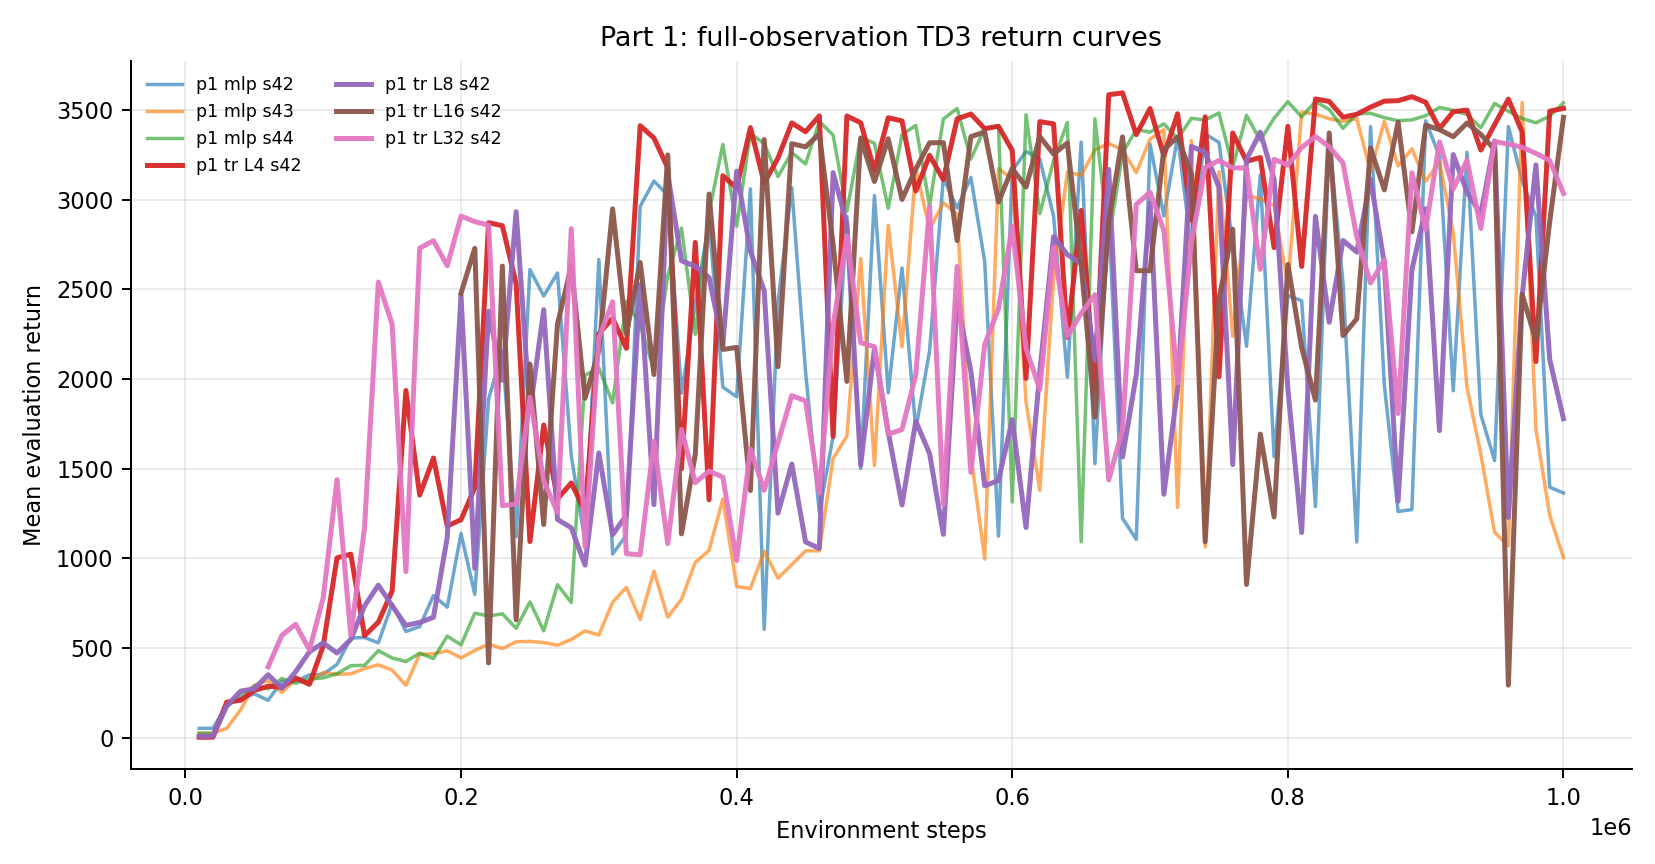
\includegraphics[width=\textwidth]{figures/fig_p1_context_sweep.png}
\caption{Evaluation-return curves for the MLP baseline seeds and Transformer context-length sweep.}
\label{fig:p1-curves}
\end{figure}

\subsection{Part 2: Partial Observability}

Under hidden velocities, the final Transformer run is -65.1 return points relative to the MLP run, which means memory did not reliably convert the available position history into a better final controller in this execution. Under delayed rewards, the $K=10$ setting is strong for both agents, with the Transformer differing from the MLP by -53.1 final-return points. For $K=30$, both policies are much weaker, and the Transformer is only moderately better than the MLP. Noisy observations remain difficult for both models, especially compared with full-observation Hopper.

\begin{table}[!htbp]
\centering
\small
\caption{MLP versus Transformer TD3 under independent partial-observability modifications.}
\label{tab:pomdp-comparison}
\resizebox{\textwidth}{!}{%
\begin{tabular}{lrrrrrr}
\toprule
Setting & MLP final & Transformer final & Final delta & MLP best & Transformer best & Best delta \\
\midrule
Hidden velocities & 318.1 & 253.0 & -65.1 & 999.1 & 986.3 & -12.8 \\
Noise sigma=0.1 & 357.6 & 288.4 & -69.2 & 370.5 & 300.5 & -69.9 \\
Noise sigma=0.3 & 234.3 & 325.0 & 90.7 & 266.7 & 405.5 & 138.8 \\
Delay K=10 & 3007.5 & 2954.4 & -53.1 & 3309.7 & 3158.5 & -151.2 \\
Delay K=30 & 390.4 & 511.8 & 121.4 & 1072.6 & 571.9 & -500.7 \\
\bottomrule
\end{tabular}
}
\end{table}

\begin{figure}[!htbp]
\centering
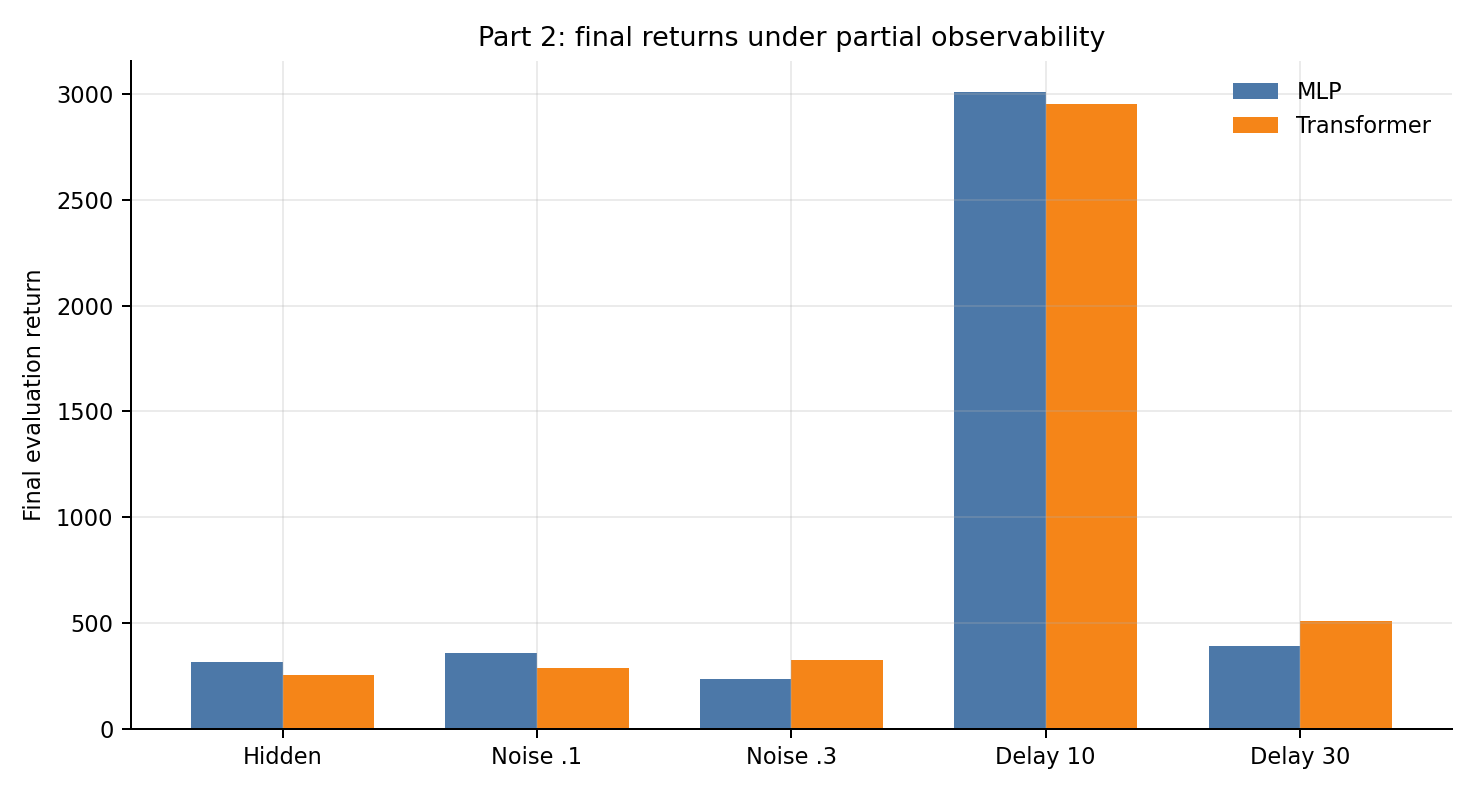
\includegraphics[width=0.88\textwidth]{figures/fig_p2_pomdp_bars.png}
\caption{Final returns for MLP and Transformer policies under independent POMDP stressors.}
\label{fig:pomdp-bars}
\end{figure}

\subsection{RLHF-Style Learned Reward}

The learned-reward run is substantially worse than the ground-truth Transformer baseline, but this comparison should be interpreted as an implementation-level learned-reward baseline. The code was intended to label preferences using ground-truth segment returns, but upon review, after warm-up the replay buffer stores learned reward predictions for TD3, so later preference updates can be partially contaminated by the model's own earlier predictions. This makes reward-model drift and self-reinforcing misranking plausible contributors to the large performance gap.

\begin{table}[!htbp]
\centering
\small
\caption{Learned-reward RLHF run compared against ground-truth-reward Transformer runs.}
\label{tab:rlhf-comparison}
\resizebox{\textwidth}{!}{%
\begin{tabular}{lrrrrrr}
\toprule
Comparison & GT final & RLHF final & Final drop & GT best & RLHF best & Reward loss \\
\midrule
Transformer L=8 baseline & 1778.8 & 155.6 & 1623.2 & 3377.4 & 1035.3 & 0.184 \\
Attention-support full repeat & 3321.9 & 155.6 & 3166.4 & 3442.7 & 1035.3 & 0.184 \\
\bottomrule
\end{tabular}
}
\end{table}

\subsubsection{Contamination and Consequences}
Per the assignment, preference labels should be generated from ground-truth segment returns, while TD3 training should use the learned reward model as the substitute reward. In my implementation, the replay buffer stored the reward value used for TD3 updates. After warm-up, that value could be the learned reward prediction rather than the true environment reward. As a result, later preference-pair labels could be computed from replay rewards that already contain the model's own earlier predictions.

This matters because it weakens the interpretation of the RLHF comparison. The learned-reward run still tests an implementation-level learned-reward pipeline, but it is not a clean Christiano-style comparison in which ground-truth returns are used only for labels and never replaced inside the labeling source. The likely consequence is self-reinforcing reward-model error. If the reward model mis-ranks local state-action decisions early, later preference updates may partially train on those distorted rewards, amplify critic error, and push the actor toward behavior that looks good to the learned model but not to Hopper's true return.

Therefore, I reported the gap in metrics with this caveat. The RLHF run ends at 155.6 final return and peaks at 1035.3, far below the L=8 ground-truth Transformer baseline, which ends at 1778.8 and peaks at 3377.4. A clean rerun would be the better evidence, but the finished RLHF run took 22,043 seconds, or 6.12 hours, and the L=8 ground-truth baseline took 20,459 seconds, or 5.68 hours. Given that this problem was discovered late, I was unable to provide a clean re-run.

\section{Attention Analysis}

The attention-analysis runner now completes the required Section 3 analysis. It uses the two later attention reruns, \href{https://wandb.ai/krishsachdev246-bits-pilani/saidl-rl/runs/jx1lmi8i}{\texttt{jx1lmi8i}} for the fully observable Transformer and \href{https://wandb.ai/krishsachdev246-bits-pilani/saidl-rl/runs/lap7edb6}{\texttt{lap7edb6}} for the hidden-velocity Transformer. Both runs are finished, both reached 1M environment steps, and both logged attention entropy, effective context, and lag weights across training. The runner then loaded the final Transformer checkpoints and rolled out five evaluation episodes per setting to compare mean attention weights over past timesteps.

This section should be read as raw-attention analysis, not as completed Chefer-style relevance propagation. The repository contains attribution-oriented support code, but the completed artifacts used here are attention weights, entropy summaries, and rollout comparisons. Therefore I treat the optional Chefer et al. attribution item as not counted quantitatively, while the assignment's required attention-analysis item is complete.

\begin{table}[!htbp]
\centering
\scriptsize
\caption{Completed attention-analysis runs and rollout summaries. Training entropy is logged over W\&B evaluation points; rollout return and rollout entropy are computed from five final-checkpoint episodes.}
\label{tab:attention-completed}
\resizebox{\textwidth}{!}{%
\begin{tabular}{llrllrrrrr}
\toprule
Setting & Run id & Points & Step range & Training entropy & Final effective context & History final & History best & Rollout return & Rollout entropy \\
\midrule
full & jx1lmi8i & 100 & 10000--1000000 & 2.075 $\rightarrow$ 1.531 & 4.62 & 1397.6 & 3390.0 @ 990k & 3327.7 $\pm$ 8.1 & 0.520 \\
hidden & lap7edb6 & 100 & 10000--1000000 & 2.076 $\rightarrow$ 0.919 & 2.51 & 296.4 & 993.2 @ 90k & 235.2 $\pm$ 76.8 & 0.295 \\
\bottomrule
\end{tabular}
}
\end{table}

The training curves show that both policies move away from nearly uniform attention over the eight-token context. A uniform distribution over eight positions has entropy $\log 8 \approx 2.079$, which matches the first logged values for both runs. By the final evaluation, the full-observation run falls to entropy 1.531, while the hidden-velocity run falls much further to 0.919. This means the hidden-velocity policy's attention became more sharply concentrated than the full-observation policy's attention.

\begin{figure}[!htbp]
\centering
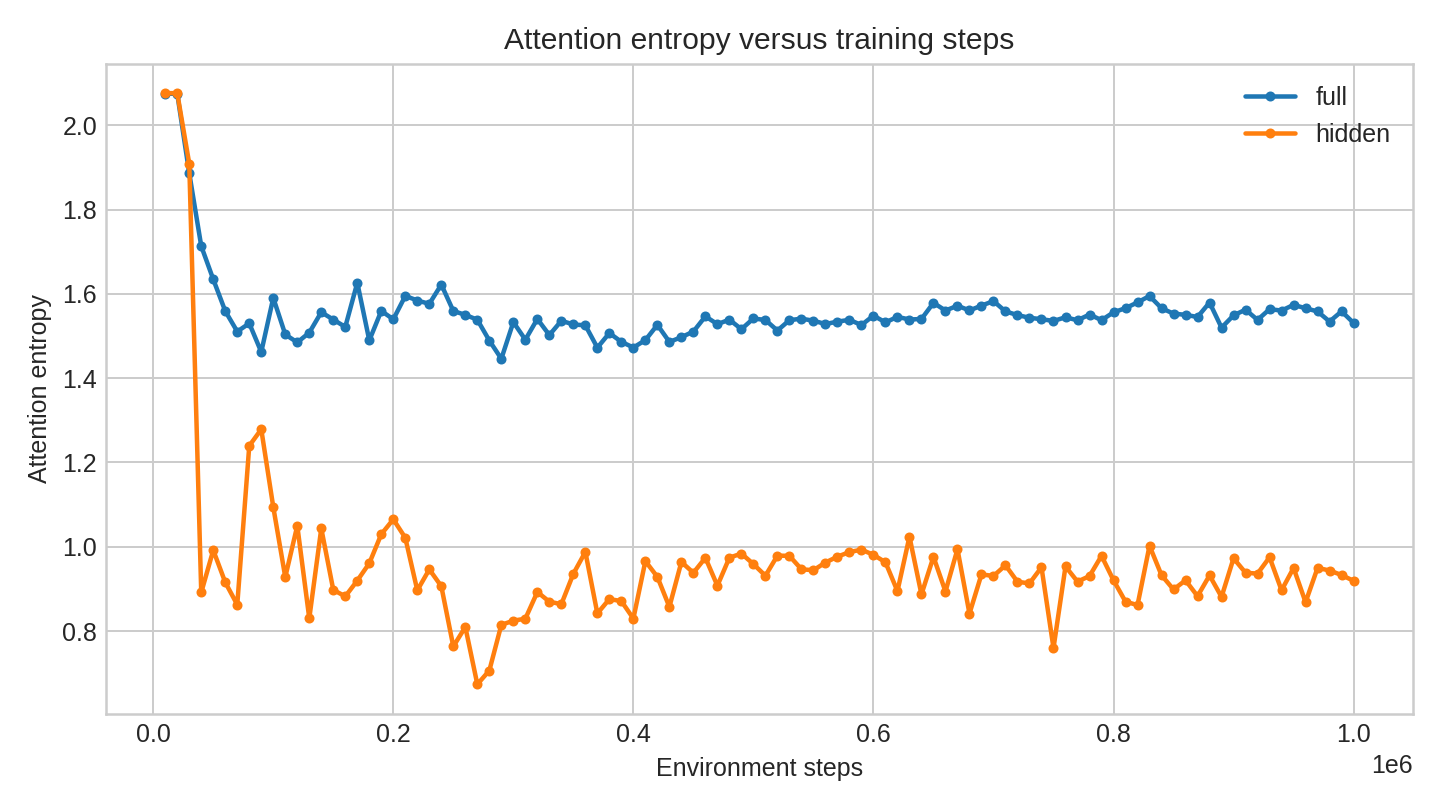
\includegraphics[width=\textwidth]{figures/fig_attention_entropy_vs_training_steps.png}
\caption{Attention entropy $H(A_t)=-\sum_j A_{t,j}\log A_{t,j}$ versus training steps for the completed full-observation and hidden-velocity attention reruns.}
\label{fig:attention-entropy-steps}
\end{figure}

\begin{figure}[!htbp]
\centering
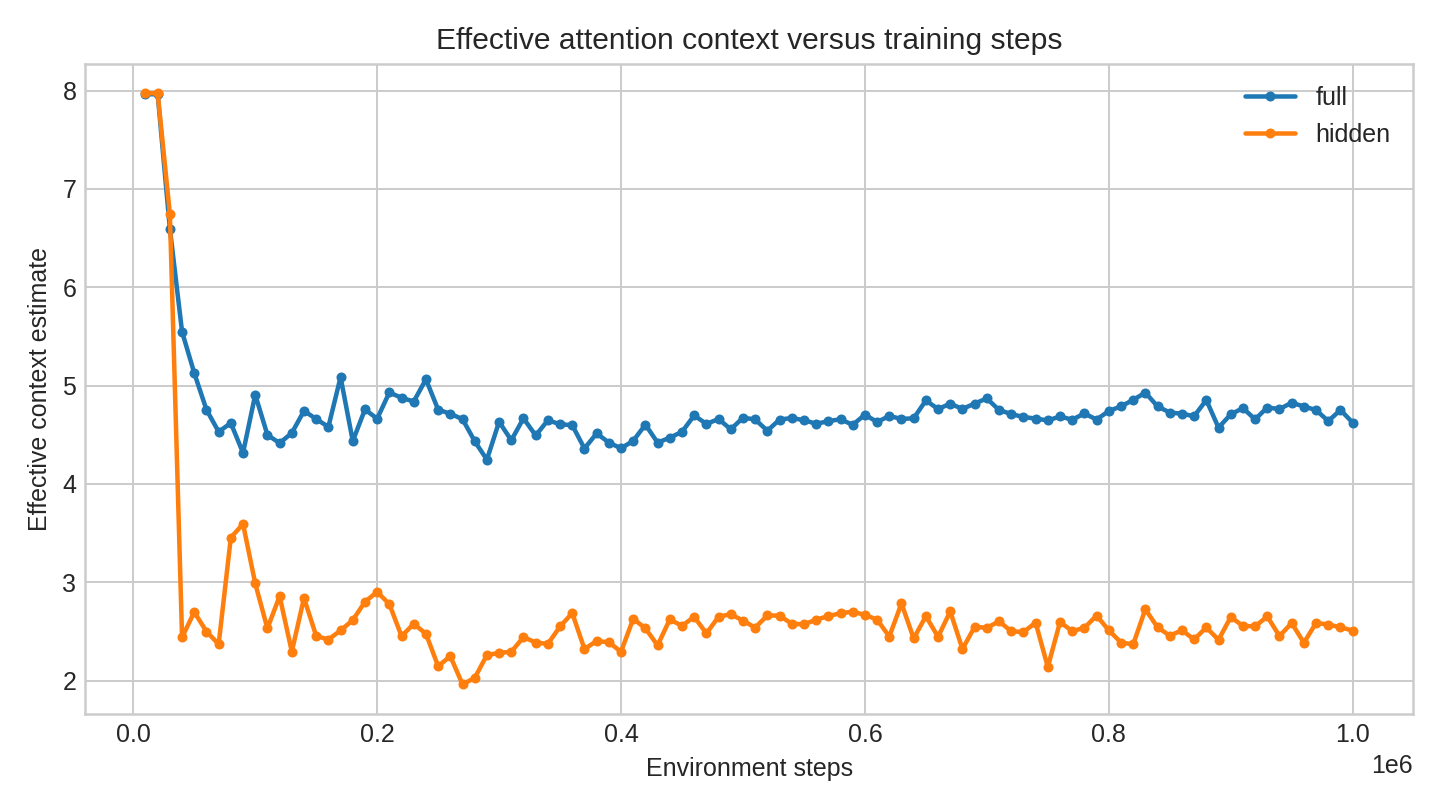
\includegraphics[width=0.88\textwidth]{figures/fig_attention_effective_context_vs_training_steps.png}
\caption{Effective context estimate over training. Lower values indicate attention concentrated on fewer timesteps.}
\label{fig:attention-effective-context}
\end{figure}

\begin{figure}[!htbp]
\centering
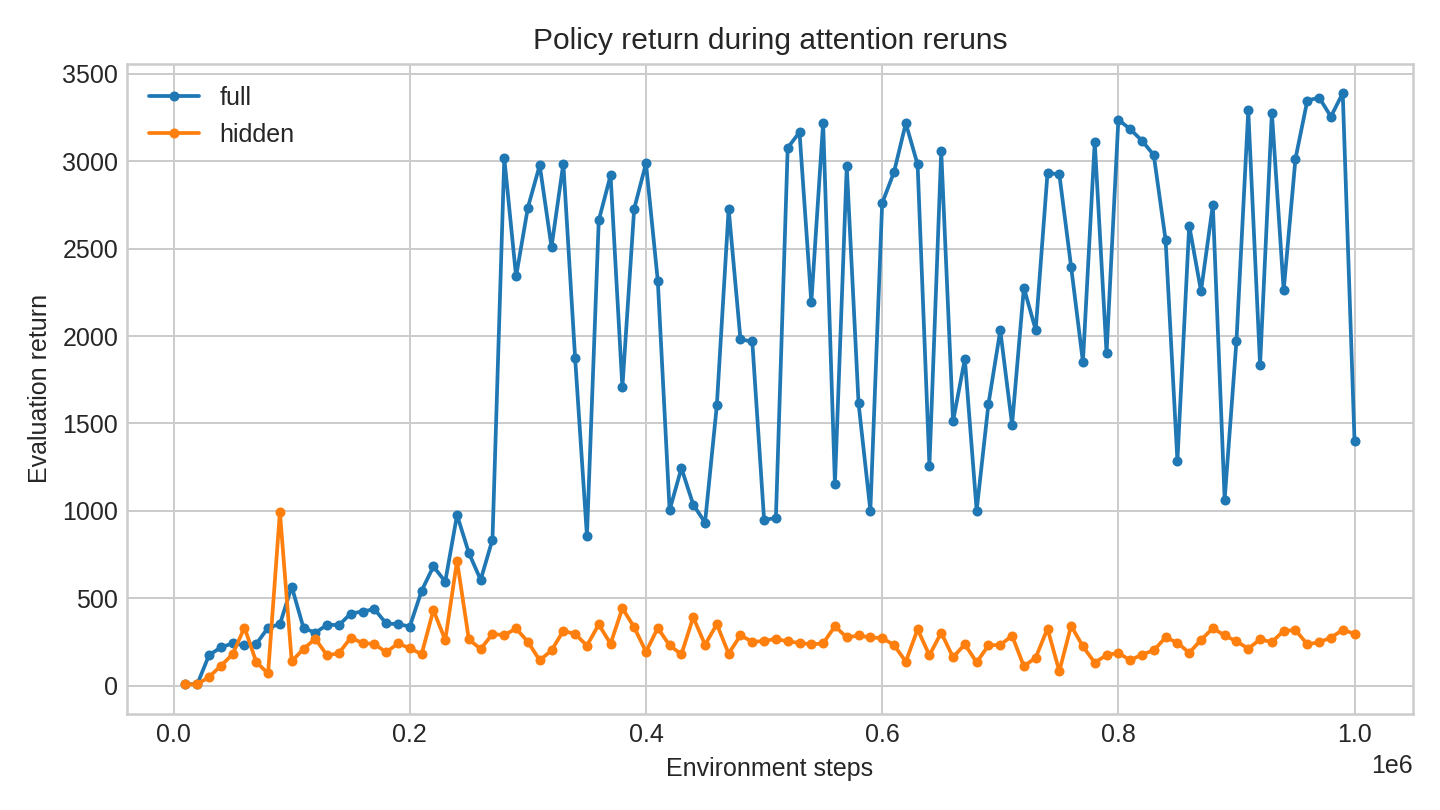
\includegraphics[width=0.88\textwidth]{figures/fig_attention_eval_return_vs_steps.png}
\caption{Evaluation return over the same training window used for the attention-entropy logs.}
\label{fig:attention-return-steps}
\end{figure}

The final lag weights make the same pattern clearer. The full-observation policy assigns 0.451 weight to the most recent token and still spreads nontrivial mass over older lags, especially lag 1 and lag 7. The hidden-velocity policy assigns 0.732 weight to lag 0 and only 0.015 to lag 1. Counterintuitively, the hidden-velocity policy did not learn a broad temporal integration pattern in this final checkpoint; it mostly collapsed onto the newest available observation-action pair, with a secondary contribution from lag 2.

\begin{table}[!htbp]
\centering
\small
\caption{Final mean attention weights by lag for the completed attention reruns.}
\label{tab:attention-final-lags}
\resizebox{\textwidth}{!}{%
\begin{tabular}{lrrrrrrrr}
\toprule
Setting & lag 0 & lag 1 & lag 2 & lag 3 & lag 4 & lag 5 & lag 6 & lag 7 \\
\midrule
full & 0.4507 & 0.1432 & 0.0768 & 0.0540 & 0.0589 & 0.0396 & 0.0809 & 0.0959 \\
hidden & 0.7322 & 0.0155 & 0.1030 & 0.0136 & 0.0207 & 0.0255 & 0.0355 & 0.0542 \\
\bottomrule
\end{tabular}
}
\end{table}

\begin{figure}[!htbp]
\centering
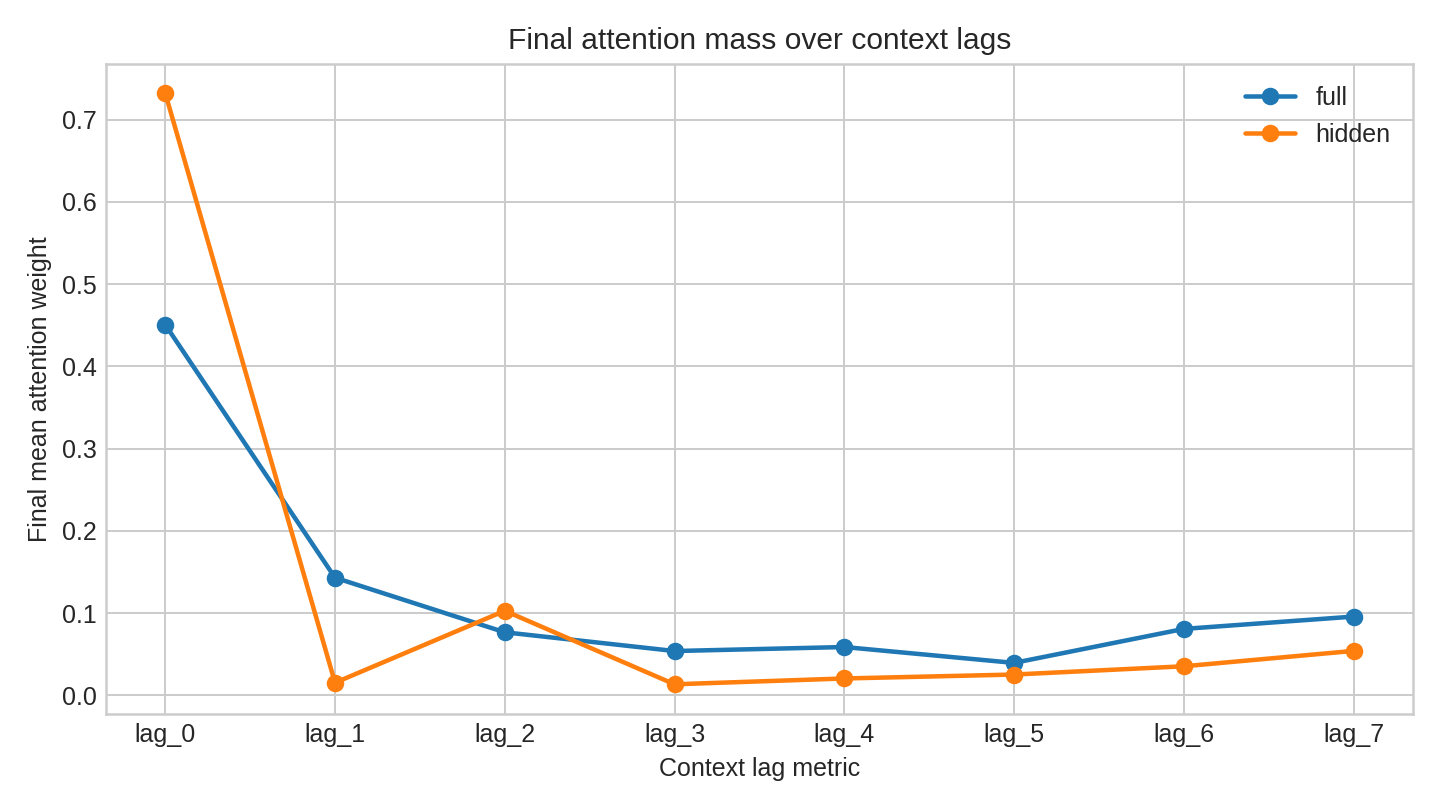
\includegraphics[width=0.88\textwidth]{figures/fig_attention_final_lag_weights.png}
\caption{Final lag weights from the completed attention reruns. Lag 0 is the most recent token in the context window.}
\label{fig:attention-final-lags}
\end{figure}

The five-episode checkpoint rollouts complete the required comparison of mean attention weights over past timesteps per decision. The full-observation checkpoint averages 3327.7 return with very low rollout variance, matching the earlier policy-quality result that full-observation Transformer control is strong. The hidden-velocity checkpoint averages only 235.2 return with higher variance. Its rollout entropy is also lower than the full-observation rollout entropy, consistent with the training-history evidence that the hidden policy concentrates attention more aggressively.

\begin{figure}[!htbp]
\centering
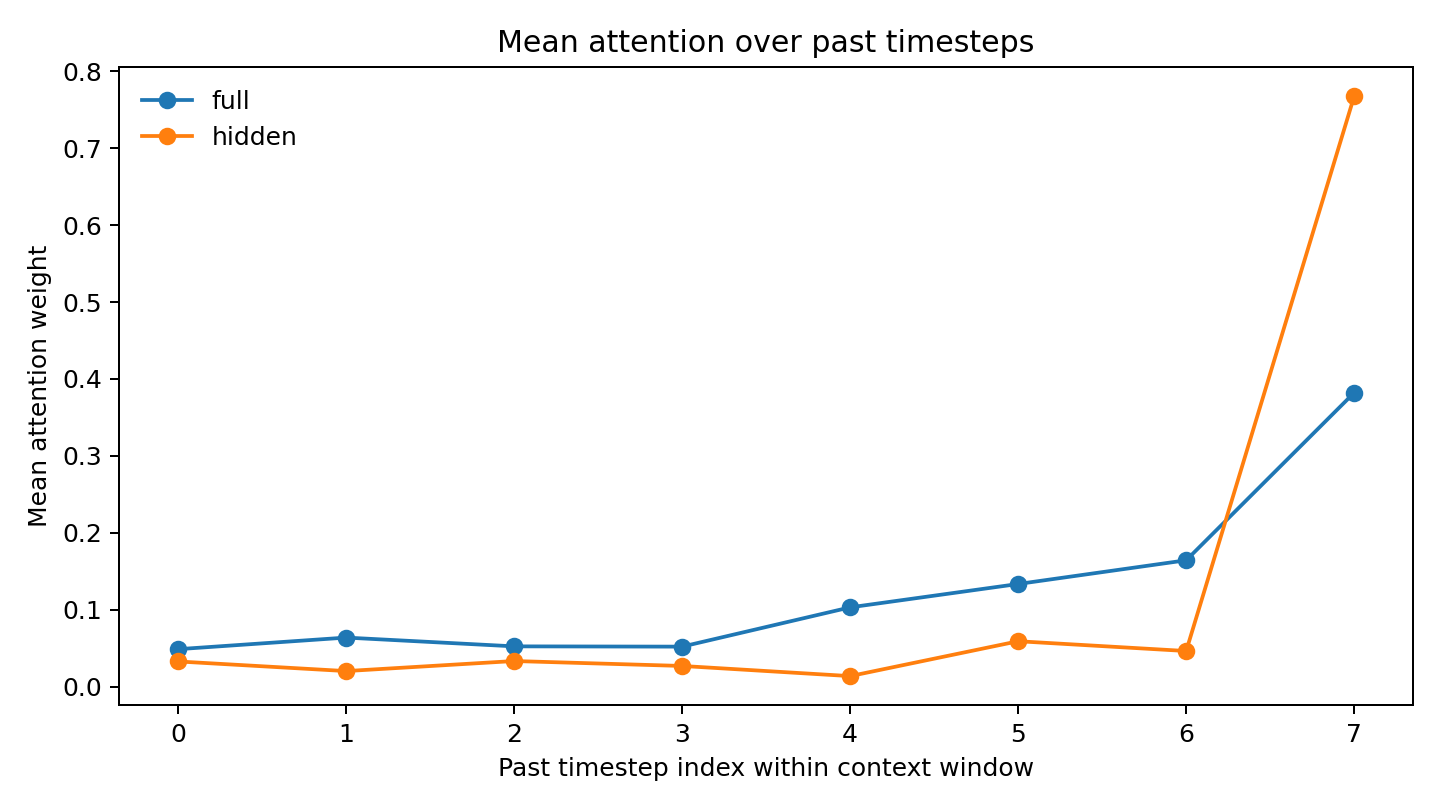
\includegraphics[width=0.88\textwidth]{figures/fig_attention_rollout_mean_weights.png}
\caption{Mean attention weights over the context window during five final-checkpoint rollout episodes. This directly addresses the assignment request to compare full observation against hidden velocity.}
\label{fig:attention-rollout-mean}
\end{figure}

\begin{figure}[!htbp]
\centering
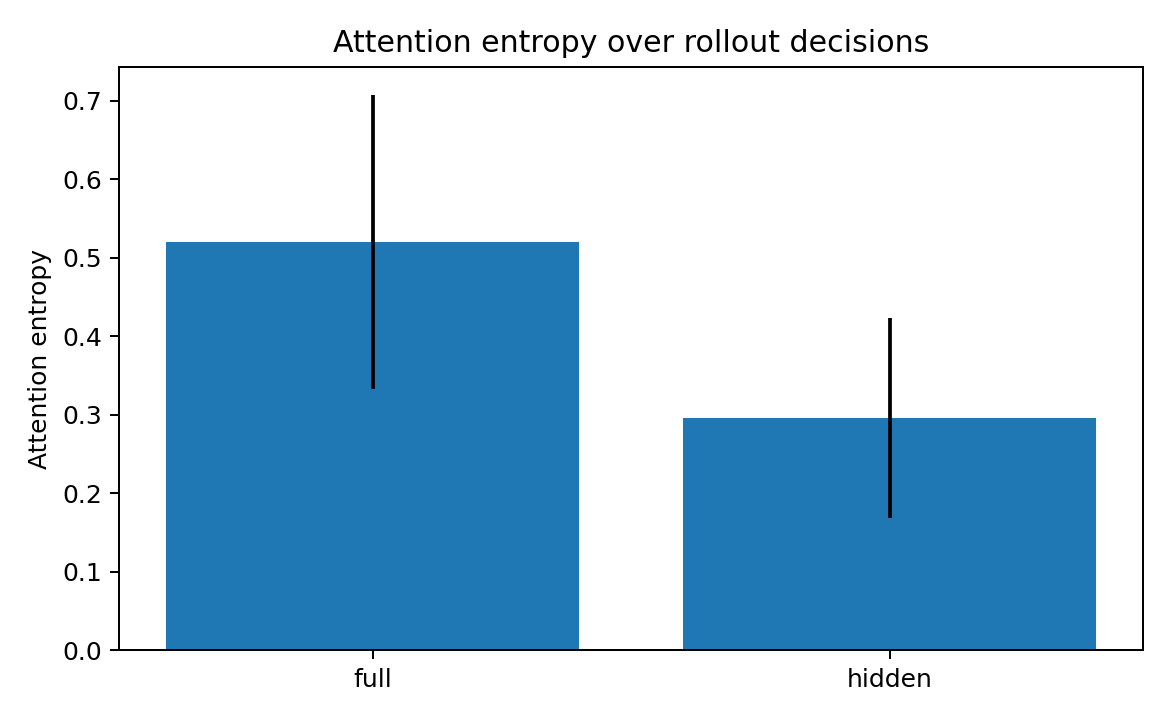
\includegraphics[width=0.72\textwidth]{figures/fig_attention_rollout_entropy.png}
\caption{Rollout attention entropy over five final-checkpoint episodes. The hidden-velocity checkpoint is more concentrated and lower-return.}
\label{fig:attention-rollout-entropy}
\end{figure}

The important interpretation is that attention concentration is not automatically evidence of a better memory policy. The full-observation run has higher final entropy, higher effective context, and much stronger rollout return. The hidden-velocity run has lower entropy and stronger concentration on the latest token, but its returns remain low. In this implementation, the attention plots show that the Transformer actor exposes a measurable temporal-attention mechanism, but they also show that the hidden-velocity setting did not reliably exploit the whole context window to reconstruct velocity.

\section{Bonus RL Experiments}

The bonus runs address three additional questions from the assignment PDF: positional encodings under hidden velocity, a combined POMDP stressor, and sequence-model policy alternatives such as Algorithm Distillation or xLSTM. The finished evidence at the time of export covers the positional-encoding ablation and the combined POMDP. I do not count AD or xLSTM because no finished metric row for those experiments is present in the current W\&B export (the runs could not be finished on time).

\subsection{Hidden-Velocity Positional Encoding Ablation}

The first set of finished positional runs used the earlier flat-critic setup and all ended in a narrow low-return band: learned absolute positions finished at 252.3, sinusoidal at 249.8, and RoPE at 248.0. Later stability-tagged (minor stability improvements made) flat-critic reruns did not materially improve the final returns for learned or sinusoidal encodings, although they did reveal high transient peaks. The latest finished stabilized runs change the result because the critic is history-conditioned. Learned absolute positions rise to 727.8 final return, sinusoidal rises to 900.0, and RoPE reaches 1109.3.

\begin{table}[!htbp]
\centering
\scriptsize
\caption{Bonus positional ablation under hidden velocity. The latest selected row is the newest finished run for each exact stabilized experiment name.}
\label{tab:bonus-positional}
\resizebox{\textwidth}{!}{%
\begin{tabular}{llrrrrrrl}
\toprule
Variant & Earlier comparator & Earlier final & Earlier best & Earlier gap & Latest final & Latest best & Latest gap & Main reading \\
\midrule
Learned & same-name flat critic, \texttt{f6ruiao3} & 190.5 & 634.2 & -443.7 & 727.8 & 862.4 & -134.6 & Clear final-return improvement and smaller collapse gap \\
Sinusoidal & same-name flat critic, \texttt{5u0bp2ea} & 201.3 & 897.0 & -695.7 & 900.0 & 1567.0 & -667.0 & Large peak and final gain, but instability remains high \\
RoPE & earlier RoPE flat run, \texttt{ok1zy14g} & 248.0 & 248.0 & 0.0 & 1109.3 & 1266.0 & -156.7 & Best final return; no finished same-name stable predecessor was available \\
\bottomrule
\end{tabular}
}
\end{table}

\begin{figure}[!htbp]
\centering
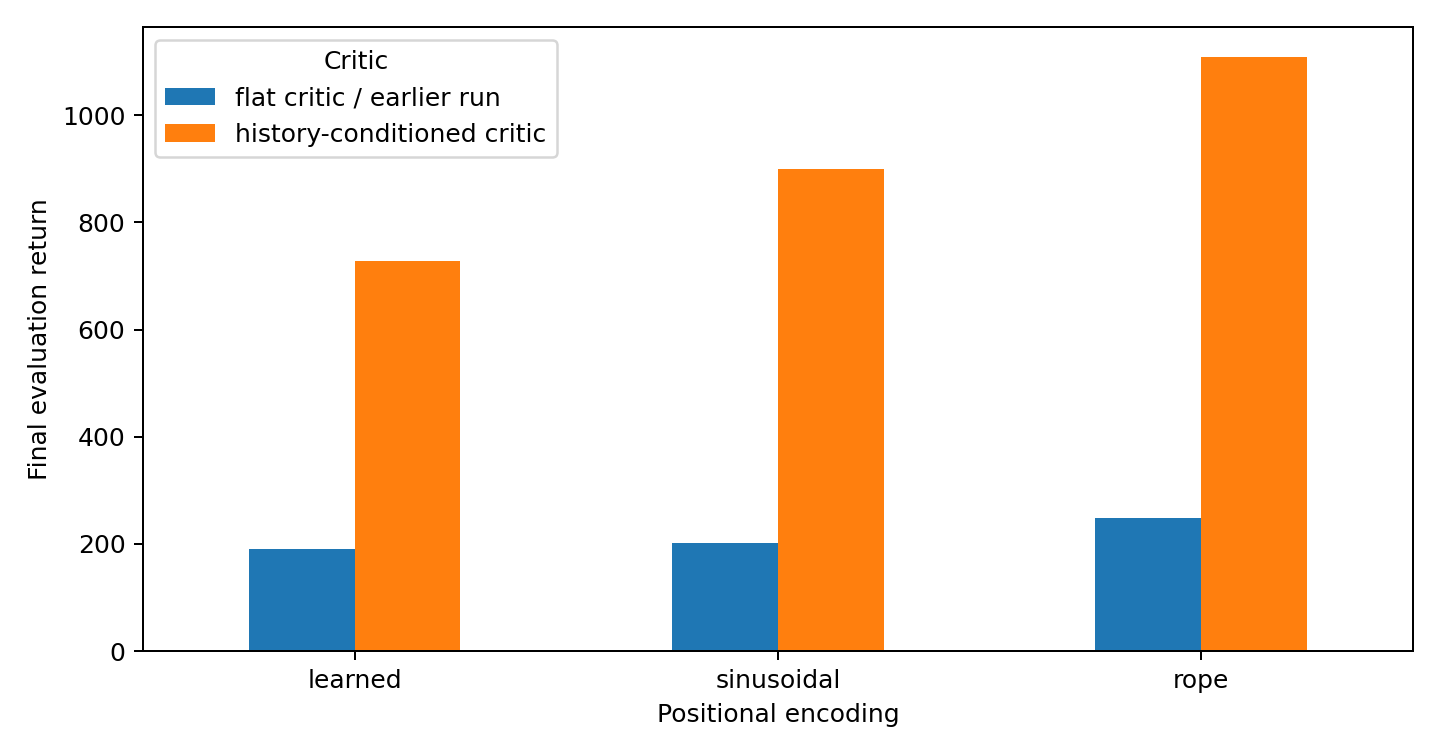
\includegraphics[width=0.88\textwidth]{figures/fig_rl_bonus_positional_critic_comparison.png}
\caption{Final returns for the latest flat-critic positional runs versus the latest history-conditioned critic runs.}
\label{fig:bonus-positional-critic}
\end{figure}

The pre-stability positional runs were suspiciously similar, clustering around final returns of roughly 250 despite using different positional encodings. That pattern suggested that the bottleneck could not have been the positional encoding alone, and once the critic receives temporal context, the positional variants separate clearly. RoPE is the best final controller, sinusoidal has the highest peak, and learned absolute positions improve but remain the weakest of the three.

The required hidden-velocity Transformer ends at 253.0 with best return 986.3, while the required hidden-velocity MLP ends at 318.1 with best return 999.1. The latest bonus RoPE run exceeds both required hidden-velocity final returns and also exceeds their best returns. Sinusoidal and learned absolute positions also beat the required hidden-velocity final returns, although learned does not beat the required best checkpoints.
\subsection{Combined POMDP}

The combined POMDP run applies hidden velocities, observation noise with $\sigma=0.1$, and delayed rewards with $K=10$ in the same Hopper task. The newest finished run, \href{https://wandb.ai/krishsachdev246-bits-pilani/saidl-rl/runs/86ypnkri}{run \texttt{86ypnkri}}, reaches final return 213.2 and best return 251.6 at step 975k. Its best-final gap is only -38.4, so the run is relatively stable, but the absolute policy quality is low.

\begin{table}[!htbp]
\centering
\small
\caption{Combined POMDP compared with the closest required single-stressor Transformer runs.}
\label{tab:bonus-combined}
\resizebox{\textwidth}{!}{%
\begin{tabular}{lrrrr}
\toprule
Setting & Final return & Best return & Best step & Best-final gap \\
\midrule
Hidden velocity Transformer & 253.0 & 986.3 & 100000 & -733.3 \\
Noise $\sigma=0.1$ Transformer & 288.4 & 300.5 & 890000 & -12.1 \\
Delay $K=10$ Transformer & 2954.4 & 3158.5 & 840000 & -204.1 \\
Combined hidden + noise + delay, L=32 & 213.2 & 251.6 & 975000 & -38.4 \\
\bottomrule
\end{tabular}
}
\end{table}

This result is likely due to unfavorable interaction between the stressors. Delay $K=10$ alone is a high-return task for both the MLP and Transformer required runs. Once hidden velocities and noise are added, the combined task drops below the individual hidden-velocity and noisy-observation Transformer finals. The policy remains relatively stable but never reaches high-returns. Evidence points to simultaneous partial observability and reward-delay pressure being much harder than any single variant tested in the required suite.

\subsection{Algorithm Distillation and xLSTM Boundary}

Algorithm Distillation and xLSTM remain implementation targets that could not be cleanly finished within the timeframe. The report includes their code and notebook support in the repository, but without a finished W\&B metric row I do not place them in the quantitative comparison. 

\begin{figure}[!htbp]
\centering
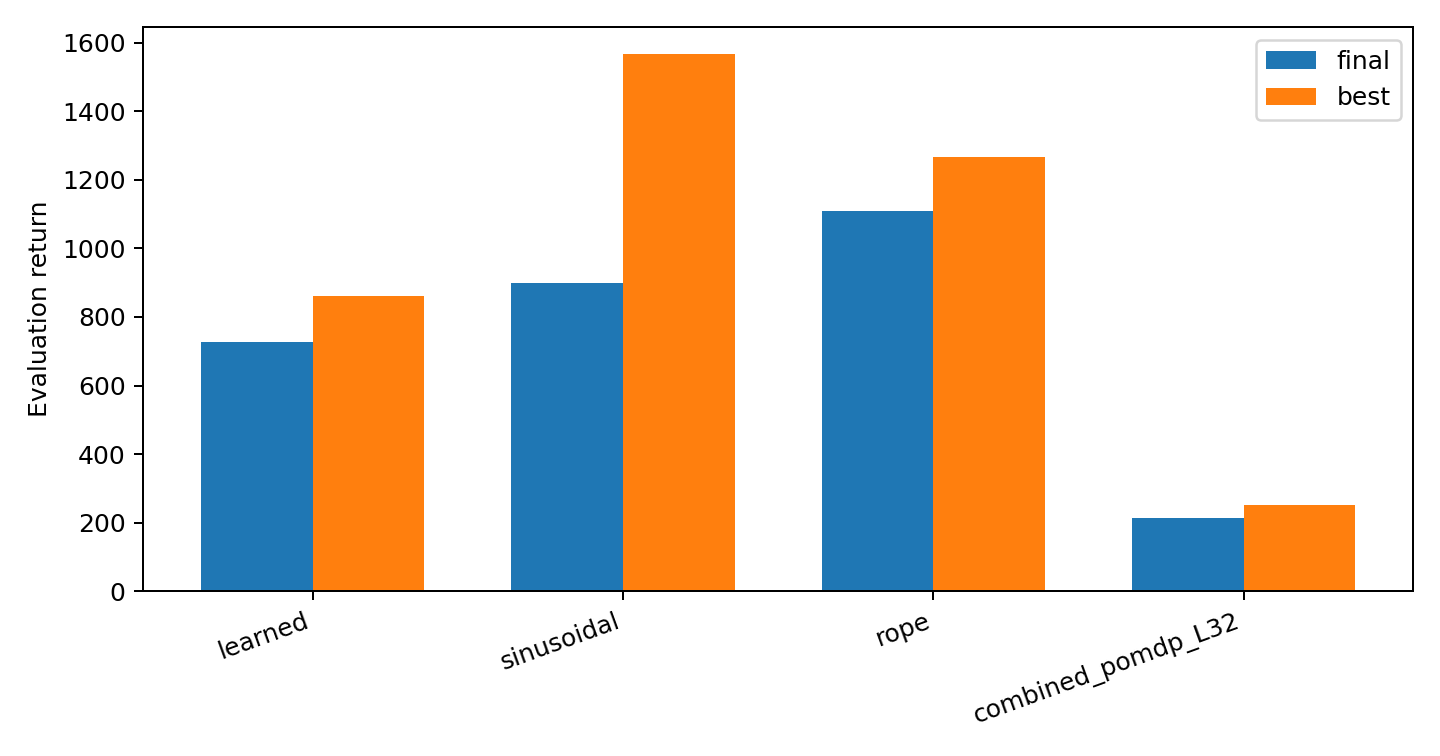
\includegraphics[width=0.88\textwidth]{figures/fig_rl_bonus_latest_final_best.png}
\caption{Final and best returns for the newest finished bonus runs counted in this report.}
\label{fig:bonus-final-best}
\end{figure}

\section{Stability, Undertraining, and Checkpoint Choice}

A major concern I faced was instability after learning: 8 selected required runs are flagged by a conservative late-deterioration threshold, with the clearest cases being p1 mlp s42, p1 mlp s43, p1 tr L8 s42, p2 hidden mlp s42, p2 hidden tr s42, p2 delay 30 mlp s42, p2 rlhf tr s42, p3 attn hidden s42. The bonus positional runs sharpen the same point. Sinusoidal with the history-conditioned critic reaches a very strong best return of 1567.0 but ends at 900.0, while RoPE has a lower peak than sinusoidal but the best final return and a much smaller collapse gap. This is why the report keeps final and best returns separate.

The likely culprits I found were characterized as "standard off-policy" actor-critic failures in other research: critic drift, extrapolation error from replay, bootstrapping noise, actor updates exploiting Q-function mistakes, and distribution shift as the learned policy changes. The POMDP wrappers may have added extra stress because noisy, delayed, or incomplete observations weaken the Markov assumption. Transformer policies added sensitivity in my opinion, I figure attention may give the actor a larger function class that may overfit critic errors.

Practical remedies I found for these were save and report best-evaluation checkpoints in addition to final checkpoints, early-stop or select by validation return when compute is limited, run more seeds for high-variance settings, tune actor and critic learning rates separately, monitor Q-value scale and critic losses, increase evaluation frequency near peaks, and make target-policy updates more conservative in unstable settings. For this report I elected to report final return for strict end-of-run comparison, best return for learned capability, and the gap as a measure of run stability.

\begin{figure}[!htbp]
\centering  
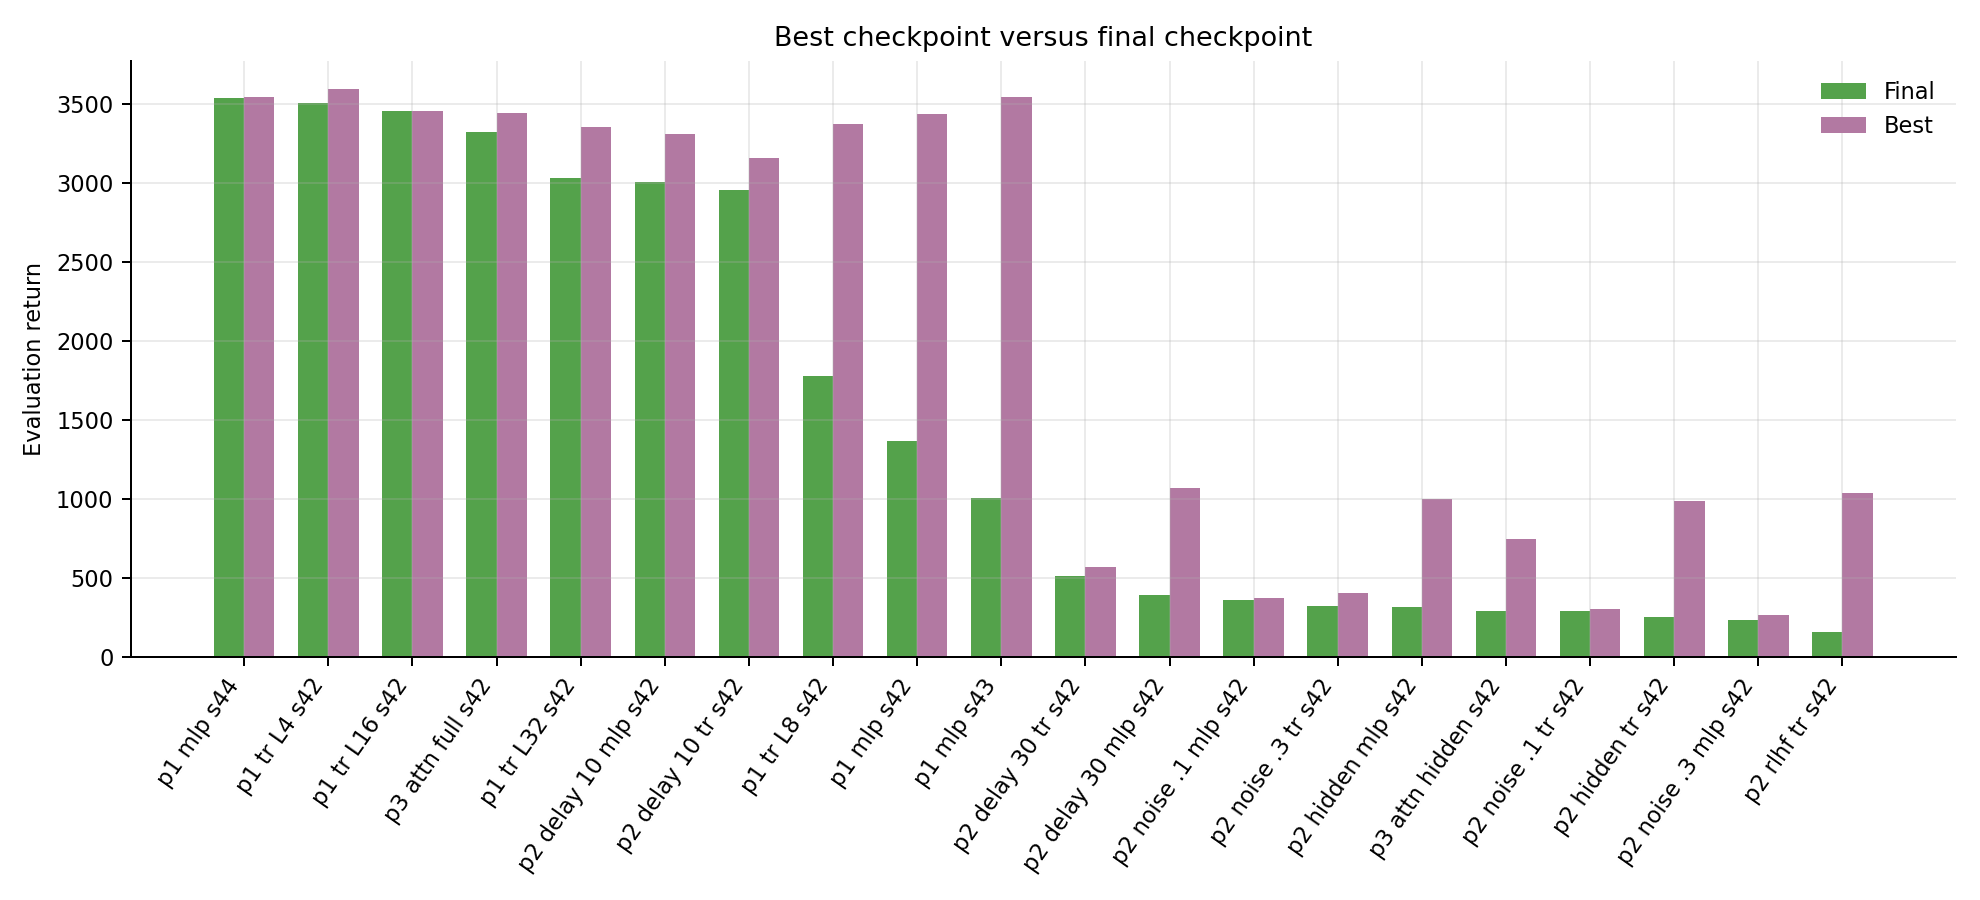
\includegraphics[width=\textwidth]{figures/fig_best_vs_final.png}
\caption{Final checkpoint return compared with best logged checkpoint return for every successful required run.}
\label{fig:best-final}
\end{figure}

\begin{figure}[!htbp]
\centering
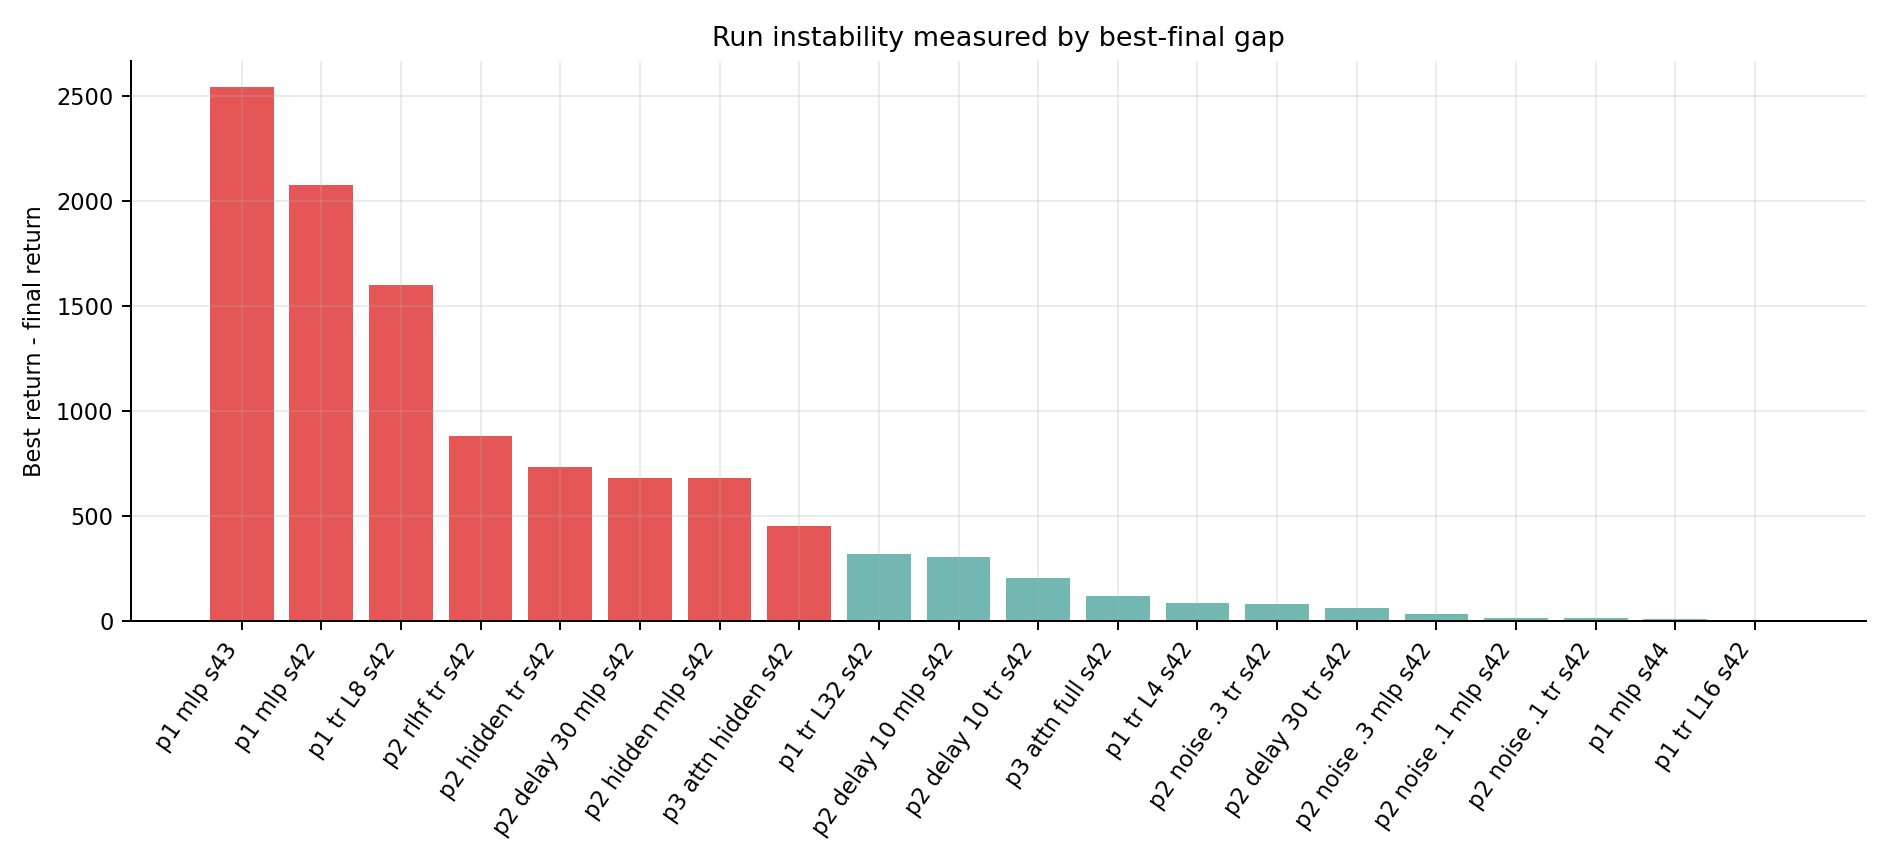
\includegraphics[width=\textwidth]{figures/fig_stability_gap.png}
\caption{Best-final return gap. Larger bars indicate stronger late deterioration after a better earlier checkpoint.}
\label{fig:stability-gap}
\end{figure}

\section{Practical Implications}

The main practical implication is that memory in the actor is useful only when the rest of the actor-critic system can use it reliably. The Transformer actor is competitive in full observation and delayed reward settings, but hidden velocity and noisy observation settings show deterioration. Temporal context alone may not guarantee a better final controller. For the bonus runs, once the critic is also history-conditioned, the hidden-velocity positional runs improve substantially and the positional encodings separate more clearly. This suggests that sequence actors and memoryless critics can create an information mismatch in POMDP-style settings.

For applied RL, instability is concerning. A controller that reaches a good checkpoint and later deteriorates would be risky in a real deployment unless checkpoints are selected by evaluation return, monitored continuously, and protected against critic drift. It's also crucial to note learned-reward systems must keep the ground-truth labeling source separate from learned rewards, otherwise preference learning can become self-referential and the comparison is no longer faithful.

\section{Hardware and Runtime Caveat}

The final suite used both P100 and T4 hardware because of issues with Kaggle availability. Runtime therefore should not be read as an architecture-speed benchmark. T4 and P100 differ in GPU generation, available kernels, and, in this Kaggle setup, GPU count. The evaluation returns remain meaningful for algorithmic comparison because the environment, seeds, step budget, and training commands are the quantities that define the RL experiment.

\begin{figure}[!htbp]
\centering
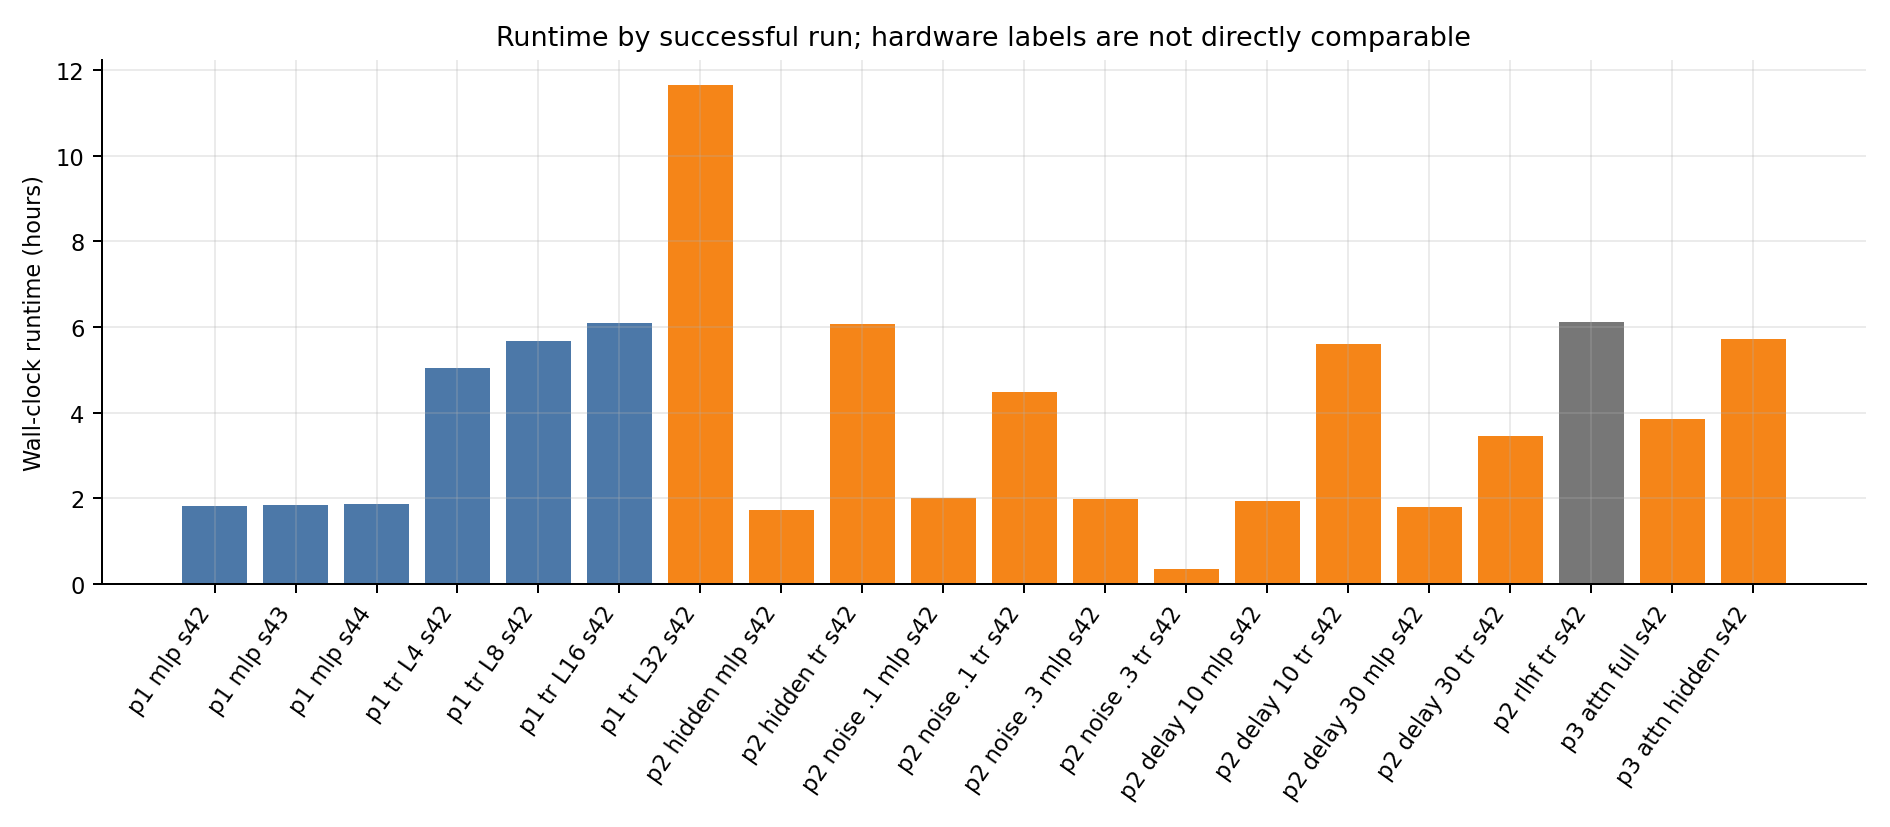
\includegraphics[width=\textwidth]{figures/fig_runtime_hardware.png}
\caption{Wall-clock runtimes for successful runs. These values document execution cost, not a controlled hardware benchmark.}
\label{fig:runtime-hardware}
\end{figure}

\section{Conclusion}

The required RL suite was completed with all 20 required final-tagged experiments present as successful W\&B runs, and the attention-analysis rerun now provides the missing entropy histories and five-episode rollout comparison. The strongest required result is that memory-based policies can be competitive and sometimes strong, especially in full-observation and delayed-reward settings. Under hidden velocity, the latest history-conditioned critic runs separate the positional encodings and improve final returns substantially over the earlier flat-critic attempts. RoPE gives the strongest final bonus return, sinusoidal gives the strongest bonus peak, and learned absolute positions improve but remain behind both.

The completed attention section shows that both Transformer policies move away from uniform attention, but the hidden-velocity policy concentrates most strongly on the newest token and still remains low-return. That is useful evidence against treating low entropy as automatically good memory use. The combined POMDP run is stable but low-return, showing that hidden state, noisy observations, and delayed rewards together are substantially harder than the single-stressor settings. The most important reporting lesson is to separate three ideas that are easy to mix up. Final evaluation return is the strict end-of-training result, best evaluation return tells whether the method learned a good policy at any point, and the best-final gap measures stability.

\appendix
\section{Selected W\&B Runs}
\footnotesize
\begin{itemize}
\item \href{https://wandb.ai/krishsachdev246-bits-pilani/saidl-rl/runs/orduqlzt}{\texttt{rl\_p1\_mlp\_seed42}} (run id \texttt{orduqlzt}, 2026-05-23T09:21:36Z; Part 1, MLP, Full; final 1364.2, best 3440.7, hardware Tesla P100-PCIE-16GB)
\item \href{https://wandb.ai/krishsachdev246-bits-pilani/saidl-rl/runs/12tb4cex}{\texttt{rl\_p1\_mlp\_seed43}} (run id \texttt{12tb4cex}, 2026-05-23T11:10:50Z; Part 1, MLP, Full; final 1004.3, best 3543.1, hardware Tesla P100-PCIE-16GB)
\item \href{https://wandb.ai/krishsachdev246-bits-pilani/saidl-rl/runs/xe1bvoqz}{\texttt{rl\_p1\_mlp\_seed44}} (run id \texttt{xe1bvoqz}, 2026-05-23T13:01:35Z; Part 1, MLP, Full; final 3540.2, best 3547.8, hardware Tesla P100-PCIE-16GB)
\item \href{https://wandb.ai/krishsachdev246-bits-pilani/saidl-rl/runs/k4mmxrji}{\texttt{rl\_p1\_tr\_L4\_seed42}} (run id \texttt{k4mmxrji}, 2026-05-23T20:03:28Z; Part 1, Transformer, Full; final 3509.9, best 3596.1, hardware Tesla P100-PCIE-16GB)
\item \href{https://wandb.ai/krishsachdev246-bits-pilani/saidl-rl/runs/jcs1nkci}{\texttt{rl\_p1\_tr\_L8\_seed42}} (run id \texttt{jcs1nkci}, 2026-05-24T01:05:56Z; Part 1, Transformer, Full; final 1778.8, best 3377.4, hardware Tesla P100-PCIE-16GB)
\item \href{https://wandb.ai/krishsachdev246-bits-pilani/saidl-rl/runs/d6s0vtx6}{\texttt{rl\_p1\_tr\_L16\_seed42}} (run id \texttt{d6s0vtx6}, 2026-05-24T10:58:11Z; Part 1, Transformer, Full; final 3459.6, best 3459.6, hardware Tesla P100-PCIE-16GB)
\item \href{https://wandb.ai/krishsachdev246-bits-pilani/saidl-rl/runs/tc91exur}{\texttt{rl\_p1\_tr\_L32\_seed42}} (run id \texttt{tc91exur}, 2026-05-25T09:27:28Z; Part 1, Transformer, Full; final 3035.7, best 3353.2, hardware Tesla T4 x2)
\item \href{https://wandb.ai/krishsachdev246-bits-pilani/saidl-rl/runs/96m7x5eb}{\texttt{rl\_p2\_hidden\_vel\_mlp\_seed42}} (run id \texttt{96m7x5eb}, 2026-05-26T07:57:53Z; Part 2a, MLP, Hidden velocity; final 318.1, best 999.1, hardware Tesla T4 x2)
\item \href{https://wandb.ai/krishsachdev246-bits-pilani/saidl-rl/runs/4hl8amlc}{\texttt{rl\_p2\_hidden\_vel\_tr\_seed42}} (run id \texttt{4hl8amlc}, 2026-05-26T09:41:52Z; Part 2a, Transformer, Hidden velocity; final 253.0, best 986.3, hardware Tesla T4 x2)
\item \href{https://wandb.ai/krishsachdev246-bits-pilani/saidl-rl/runs/lgmxbqai}{\texttt{rl\_p2\_noise01\_mlp\_seed42}} (run id \texttt{lgmxbqai}, 2026-05-26T15:45:40Z; Part 2b, MLP, Noisy; final 357.6, best 370.5, hardware Tesla T4 x2)
\item \href{https://wandb.ai/krishsachdev246-bits-pilani/saidl-rl/runs/3lt7il9g}{\texttt{rl\_p2\_noise01\_tr\_seed42}} (run id \texttt{3lt7il9g}, 2026-05-27T16:57:39Z; Part 2b, Transformer, Noisy; final 288.4, best 300.5, hardware Tesla T4 x2)
\item \href{https://wandb.ai/krishsachdev246-bits-pilani/saidl-rl/runs/anlzqstp}{\texttt{rl\_p2\_noise03\_mlp\_seed42}} (run id \texttt{anlzqstp}, 2026-05-27T21:26:17Z; Part 2b, MLP, Noisy; final 234.3, best 266.7, hardware Tesla T4 x2)
\item \href{https://wandb.ai/krishsachdev246-bits-pilani/saidl-rl/runs/f4lc5xjg}{\texttt{rl\_p2\_noise03\_tr\_seed42}} (run id \texttt{f4lc5xjg}, 2026-05-28T05:24:55Z; Part 2b, Transformer, Noisy; final 325.0, best 405.5, hardware Tesla T4 x2)
\item \href{https://wandb.ai/krishsachdev246-bits-pilani/saidl-rl/runs/523e0uha}{\texttt{rl\_p2\_delay10\_mlp\_seed42}} (run id \texttt{523e0uha}, 2026-05-28T05:46:42Z; Part 2c, MLP, Delayed reward; final 3007.5, best 3309.7, hardware Tesla T4 x2)
\item \href{https://wandb.ai/krishsachdev246-bits-pilani/saidl-rl/runs/hfiawzrg}{\texttt{rl\_p2\_delay10\_tr\_seed42}} (run id \texttt{hfiawzrg}, 2026-05-28T07:42:38Z; Part 2c, Transformer, Delayed reward; final 2954.4, best 3158.5, hardware Tesla T4 x2)
\item \href{https://wandb.ai/krishsachdev246-bits-pilani/saidl-rl/runs/15bzu83r}{\texttt{rl\_p2\_delay30\_mlp\_seed42}} (run id \texttt{15bzu83r}, 2026-05-28T13:19:16Z; Part 2c, MLP, Delayed reward; final 390.4, best 1072.6, hardware Tesla T4 x2)
\item \href{https://wandb.ai/krishsachdev246-bits-pilani/saidl-rl/runs/kkdfxotj}{\texttt{rl\_p2\_delay30\_tr\_seed42}} (run id \texttt{kkdfxotj}, 2026-05-28T17:58:13Z; Part 2c, Transformer, Delayed reward; final 511.8, best 571.9, hardware Tesla T4 x2)
\item \href{https://wandb.ai/krishsachdev246-bits-pilani/saidl-rl/runs/rvckskwt}{\texttt{rl\_p2\_rlhf\_tr\_seed42}} (run id \texttt{rvckskwt}, 2026-05-28T21:25:25Z; Part 2d, Transformer, Full; final 155.6, best 1035.3, hardware Unknown)
\item \href{https://wandb.ai/krishsachdev246-bits-pilani/saidl-rl/runs/78e2wcm0}{\texttt{rl\_p3\_attn\_support\_full\_seed42}} (run id \texttt{78e2wcm0}, 2026-05-29T07:34:06Z; Part 3, Transformer, Full; final 3321.9, best 3442.7, hardware Tesla T4 x2)
\item \href{https://wandb.ai/krishsachdev246-bits-pilani/saidl-rl/runs/lwsokb8n}{\texttt{rl\_p3\_attn\_support\_hidden\_seed42}} (run id \texttt{lwsokb8n}, 2026-05-29T11:25:30Z; Part 3, Transformer, Hidden velocity; final 293.6, best 745.3, hardware Tesla T4 x2)
\item Attention-analysis full rerun: \href{https://wandb.ai/krishsachdev246-bits-pilani/saidl-rl/runs/jx1lmi8i}{\texttt{rl\_p3\_attn\_support\_full\_seed42}} (run id \texttt{jx1lmi8i}; final 1397.6, best 3390.0, entropy logged across 100 points)
\item Attention-analysis hidden rerun: \href{https://wandb.ai/krishsachdev246-bits-pilani/saidl-rl/runs/lap7edb6}{\texttt{rl\_p3\_attn\_support\_hidden\_seed42}} (run id \texttt{lap7edb6}; final 296.4, best 993.2, entropy logged across 100 points)
\item Bonus positional learned latest source: \href{https://wandb.ai/krishsachdev246-bits-pilani/saidl-rl/runs/jrmialcm}{\texttt{rl\_bonus\_pos\_learned\_stable\_seed42}} (run id \texttt{jrmialcm}; final 727.8, best 862.4)
\item Bonus positional sinusoidal latest source: \href{https://wandb.ai/krishsachdev246-bits-pilani/saidl-rl/runs/ivzdtxwf}{\texttt{rl\_bonus\_pos\_sinusoidal\_stable\_seed42}} (run id \texttt{ivzdtxwf}; final 900.0, best 1567.0)
\item Bonus positional RoPE latest source: \href{https://wandb.ai/krishsachdev246-bits-pilani/saidl-rl/runs/b8n09w71}{\texttt{rl\_bonus\_pos\_rope\_stable\_seed42}} (run id \texttt{b8n09w71}; final 1109.3, best 1266.0)
\item Bonus combined POMDP latest source: \href{https://wandb.ai/krishsachdev246-bits-pilani/saidl-rl/runs/86ypnkri}{\texttt{rl\_bonus\_combined\_L32\_stable\_seed42}} (run id \texttt{86ypnkri}; final 213.2, best 251.6)
\end{itemize}
\normalsize

\section{Reproducibility Notes}
The report is backed by CSV exports and generated figures. The most important support files are:
\begin{itemize}
\item \path{rl/report/data/clean_rl_required_runs.csv}
\item \path{rl/report/data/coverage_audit.csv}
\item \path{rl/report/data/wandb_rl_runs_raw.csv}
\item \path{rl/report/data/wandb_rl_runs_last3w_nonfailed.csv}
\item \path{rl/report/tables/rl_attempt_inclusive_last3w_by_name.csv}
\item \path{rl/report/data/attention_entropy_vs_steps_full_hidden.csv}
\item \path{rl/report/data/attention_history_summary.csv}
\item \path{rl/report/data/attention_rollout_summary.csv}
\item \path{rl/report/data/attention_checkpoint_manifest.csv}
\item \path{rl/report/tables/rl_attention_completed_summary.csv}
\item \path{rl/report/data/clean_rl_bonus_runs.csv}
\item \path{rl/report/tables/rl_bonus_latest_finished_by_exact_name.csv}
\item \path{rl/report/tables/rl_bonus_same_name_instability.csv}
\item \path{rl/report/tables/rl_bonus_positional_latest_by_family.csv}
\end{itemize}
These files are included so final-return, best-return, stability-gap, hardware, resume-status, bonus-selection, and same-name instability claims can be checked without relying only on the report prose.

\begin{thebibliography}{11}
\bibitem{saidl2026} Society for Artificial Intelligence and Deep Learning. \emph{SAiDL Summer Assignment 2026}. Assignment specification, 2026.
\bibitem{td3} Scott Fujimoto, Herke van Hoof, and David Meger. Addressing Function Approximation Error in Actor-Critic Methods. ICML, 2018.
\bibitem{attention} Ashish Vaswani et al. Attention Is All You Need. NeurIPS, 2017.
\bibitem{preferences} Paul F. Christiano et al. Deep Reinforcement Learning from Human Preferences. NeurIPS, 2017.
\bibitem{chefer} Hila Chefer, Shir Gur, and Lior Wolf. Transformer Interpretability Beyond Attention Visualization. CVPR, 2021.
\bibitem{spinningup} Joshua Achiam. Spinning Up in Deep Reinforcement Learning. 2018.
\bibitem{laskin2022} Michael Laskin et al. In-context Reinforcement Learning with Algorithm Distillation. 2022.
\bibitem{beck2024} Maximilian Beck et al. xLSTM: Extended Long Short-Term Memory. 2024.
\end{thebibliography}

\end{document}
